\subsubsection{Purpose}
One of the main feature of Travlendar+ is the possibility to display into the user's events schedule which kind of means of transport the user should take to reach the location of each appointments. Particularly, a user can take public transportation by buying tickets direct from the application or by inserting his pass code. If a user should take a taxi, he can easily book it by calling the local taxi service company. 
In addition, the application allows user the possibility to locate and take a shared transport of a vehicle sharing system like bike or car, simply from the application interface.

\subsubsection{Scenario 1}
\subsubsection{Scenario 2}
\subsubsection{Use case}
The use case diagram for mobility selection is shown in Figure \ref{fig:useCaseMobility}.
\begin{figure}
	\centering
	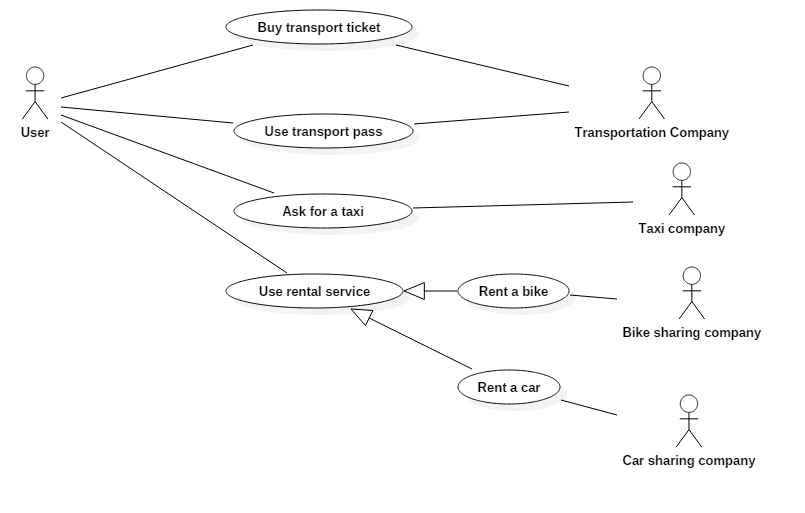
\includegraphics[width=6in]{./diagrams/TransportationUseCase.png}
	\caption{Use case diagram for mobility selection}
	\label{fig:useCaseMobility}
\end{figure}

\begin{table}
\centering
	\begin{tabular}{|c||p{0.6\textwidth}|}
    \hline
    Name & Purchase Tickets \\ \hline
    Actors & User \\  \hline
    Input condition & The user has already added at least one appointment and has been validated \\ \hline
    Flow of events & \begin{enumerate}
    \item The user may want to buy a public transport ticket
    \item The system forward the request to an external service in order to process the data and check the availability of the ticket.
    \item The external transport company API checks if there are tickets which 				are still purchased and asks to user the confirmation of buy the ticket.
    \end{enumerate} \\ \hline
     Output condition & The QR code of the tickets that he has purchased are added into the specific windows where the user can manage all his public transport ticket. \\ \hline
     Exception & The ticket may not be available for a specific means of transport (metro, bus, tram) \\ \hline
	\end{tabular}
\caption{Use case for purchase tickets}
\label{usecase_tickets}
\end{table}

\subsubsection{Sequence diagram}
The sequence diagram of the purchase tickets process is illustrated in Figure \ref{fig:useCaseMobility}.
\begin{figure}
	\centering
	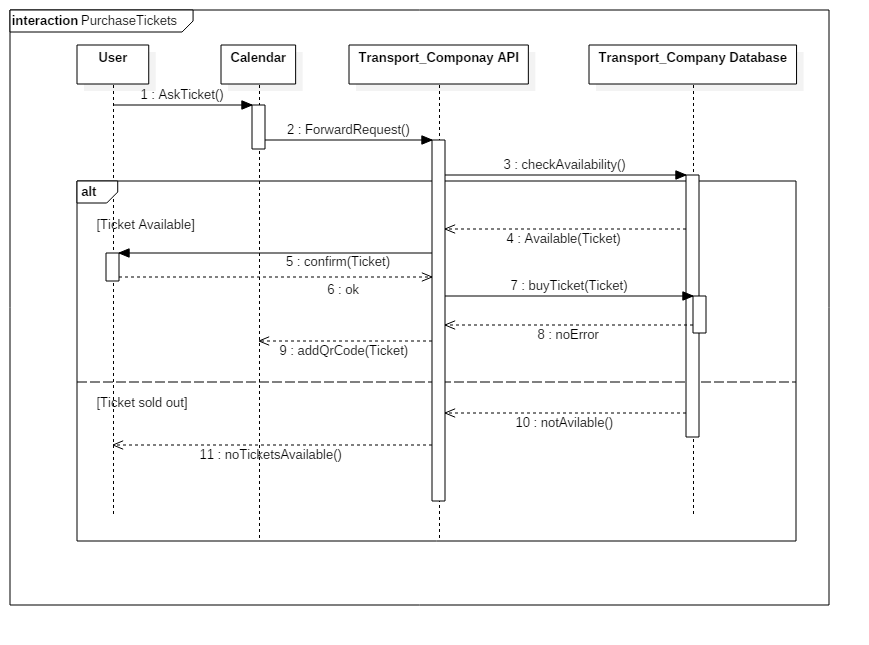
\includegraphics[width=6in]{./diagrams/PurchaseTickets.png}
	\caption{Sequence diagram: Purchase Tickets}
	\label{fig:useCaseMobility}
\end{figure}